% !TEX root = ../my-thesis.tex
%
\chapter{Introduction to Bayesian Inference}
\label{sec:bayes}
Bayesian inference is a branch of statistics that uses the Bayesian concept of probability and Bayes' theorem to investigate questions of stochastics.  Characteristic for Bayesian statistics is the consistent use of probability distributions or marginal distributions, whose form conveys the accuracy of the procedures or reliability of the data and the procedure. The Bayesian concept of probability does not presuppose infinitely repeatable random experiments, so that Bayesian methods can be used even with small data sets. A small amount of data leads to a broad probability distribution, which is not strongly localized. In the Bayesian approach, the parameters of interest are treated as random variables that are governed by their parameters, for instance the mean and standard deviation, and distributions. Bayesian inference is an essential technique in mathematical statistics and the polar opposite of the frequentist approach, in which a hypothesis is tested without being assigned a probability. In the Bayesian approach a \textit{prior} distribution $\pi\left(\pmb{\theta}\right)$ is introduced as part of the model. This distribution is intended to express a state of knowledge or ignorance about the parameters $\pmb{\theta}$ prior to obtaining the data. Using the prior distribution, the likelihood function $\pi\left(\pmb{y}|\pmb{\theta}\right)$, and the observed data $\pmb{y}$, most of the time it is possible to calculate the probability distribution $\pi\left(\pmb{\theta}\right|\pmb{y})$ of $\pmb{\theta}$ given the data $\pmb{y}$. This distribution is called the \textit{posterior} distribution of $\pmb{\theta}$ and is used to make inferences about the parameters \autocite[][6]{box2011bayesian}.
\clearpage
\section{Preliminaries}
This work follows strict notation rules to easily represent different elements such as matrices or graphs and contains frequently used abbreviations. These and some other basic concepts used in this work are introduced below. The notation follows the one used by \cite{rue2005gaussian}.
\subsection{Matrices and Vectors}
Vectors and matrices are indicated by bold notation, such as $\pmb{x}$ and $\pmb{A}$. The transpose of $\pmb{A}$ is denoted by $\pmb{A}^T$. The element in the \textit{i}th row and \textit{j}th column of $\pmb{A}$ is referenced by $A_{ij}$. This notation is used for vectors and $x_i$ denotes the \textit{i}th element of a vector. The vector $\left(x_i,x_{i+1},...,x_j\right)^T$ is abbreviated to $\pmb{x}_{i:j}$. If the columns $\pmb{A}_1, \pmb{A}_2,...,\pmb{A}_m$ of a $n\times m$ matrix $\pmb{A}$ are stacked on top of each other, this is denoted by $\hbox{vec}\left(\pmb{A}\right)=\left(\pmb{A}_1^T,\pmb{A}_2^T,...,\pmb{A}_m^T\right)$. Deleting rows and/or columns from $\pmb{A}$ creates a \textit{submatrix}. If a submatrix of a $n\times n$ matrix $\pmb{A}$ can be obtained by removing rows and columns of the same index, it is called a \textit{principal submatrix}. If this matrix can be obtained by deleting the last $n-r$ rows and columns, it is called a \textit{leading principal submatrix} of \pmb{A}. \\
A diagonal $n\times n$ matrix $\pmb{A}$ is denoted by $\hbox{diag}\left(\pmb{A}\right)$ and has the following structure:
\begin{equation*}
    \hbox{diag}\left(\pmb{A}\right)=\begin{pmatrix}
    A_{11} \\
    & \ddots \\
    &&A_{nn}
    \end{pmatrix}.
\end{equation*}
The identity matrix is denoted by $\pmb{I}$. \\
If $A_{ij}=0$ for $i<j$ or $A_{ij} = 0$ where $i>j$, then $\pmb{A}$ is called \textit{upper triangular} and \textit{lower triangular} respectively. The \textit{bandwidth} of a matrix $\pmb{A}$ is defined as $\max\left\lbrace|i-j|:A_{ij}\neq0\right\rbrace$. The \textit{lower bandwidth} is given by $\max\lbrace|i-j|:A_{ij}\neq $ $0\hbox{ and } i > j\rbrace$. $|\pmb{A}|$ denotes the \textit{determinant} of a $n\times n$ matrix $\pmb{A}$ and is equal to the product of the eigenvalues of $\pmb{A}$. The \textit{rank} of $\pmb{A}$, referenced by $\hbox{rank}\left(\pmb{A}\right)$, is the number of linearly independent rows or columns of $\pmb{A}$. The sum of the diagonal elements is called \textit{trace} of $\pmb{A}$, $\hbox{trace}\left(\pmb{A}\right)=\sum_{i}A_{ii}$.\\
Finally, '$\odot$' denotes the element-wise multiplication of two matrices of size $n\times m$, '$\oslash$' denotes the element-wise division and raising each element of a matrix $\pmb{A}$ to a scalar power uses the symbol '$\owedge$'  \autocite[][14--15]{rue2005gaussian}.
\subsection{General Notation and Abbreviations}
For $C\in\mathcal{I}=\left\lbrace1,...,n\right\rbrace$ let $\pmb{y}_C=\left\lbrace y_i:i\in C\right\rbrace$. $-C$ denotes the set $\mathcal{I-C}$ such that $\pmb{y}_{-C}=\left\lbrace y_i:i\notin C\right\rbrace$. For two sets $A$ and $B$, $A\setminus B=\left\lbrace i:i\in A \hbox{ and } i \notin B\right\rbrace$. \\
$\pi\left(\cdot\right)$ denotes the density of its arguments, for example $\pi\left(\pmb{y}\right)$ for the density of $\pmb{y}$ and $\pi\left(\pmb{y}_A|\pmb{y}_{-A}\right)$ for the conditional density of $\pmb{y}_A$, given $\pmb{y}_{-A}$. '$\sim$' is used when a variable is 'distributed' according to the law $l$ \autocite[][16]{rue2005gaussian}.
\clearpage
\section{Basic Concepts of Bayesian Theory}
To understand Bayesian theory, it is helpful to first introduce a few basic concepts, first and foremost Bayes' theorem, which is introduced in Section~\ref{sec:bayes_theorem}, one of the most famous concepts in all of statistics. Other notions that are integral to the rest of this thesis are the concept of conditional independence, undirected graphs and the computation of summary statistics, the latter of which is an essential part of the analysis section of this thesis.
\subsection{Bayes' Theorem}\label{sec:bayes_theorem}
At the heart of Bayesian inference is \textit{Bayes' theorem}, which describes the probability of an event given prior knowledge of factors that might influence the event. \\
Let $\pmb{y}^T=\left(y_1,...,y_n\right)$ be a vector of $n$ observations whose probability distribution $\pi\left(\pmb{y}|\pmb{\theta}\right)$ depends on the values of $k$ parameters $\pmb{\theta}^T=\left(\theta_1,...,\theta_k\right)$. Let $\pi\left(\pmb{\theta}\right)$ be the probability distribution of $\pmb{\pmb{\theta}}$. Then 
\begin{equation}
    \pi\left(\pmb{y}|\pmb{\theta}\right)\pi\left(\pmb{\theta}\right)=\pi\left(\pmb{y},\pmb{\theta}\right) = \pi\left(\pmb{\theta}|\pmb{y}\right)\pi\left(\pmb{y}\right).
\end{equation}
Given the observed data $\pmb{y}$, the conditional distribution of $\pmb{\theta}$ is
\begin{equation}
    \pi\left(\pmb{\theta}|\pmb{y}\right)=\frac{\pi\left(\pmb{y}|\pmb{\theta}\right)\pi\left(\pmb{\theta}\right)}{\pi\left(\pmb{y}\right)}.
\end{equation}
This last statement is known as Bayes' theorem \autocite[][]{bayes1763lii}. The \textit{prior} distribution $\pi\left(\pmb{\theta}\right)$ contains knowledge about $\pmb{\theta}$ without knowledge of the data. $\pi\left(\pmb{\theta}|\pmb{y}\right)$ contains what is known about $\pmb{\theta}$ given knowledge of the data and is the \textit{posterior} distribution of $\pmb{\theta}$ given $\pmb{y}$. \\
If $\pi\left(\pmb{y}|\pmb{\theta}\right)$ is considered as a function of $\pmb{\theta}$ instead of $\pmb{y}$, it is called the \textit{likelihood function} of $\pmb{\theta}$ given $\pmb{y}$ and can be written as $l\left(\pmb{\theta}|\pmb{y}\right)$. Thus, Bayes' theorem can be written as
\begin{equation}
    \pi\left(\pmb{\theta}|\pmb{y}\right)\propto l\left(\pmb{\theta}|\pmb{y}\right)\pi\left(\pmb{\theta}\right).
\end{equation}
It is evident that the posterior distribution of $\pmb{\theta}$ given the data $\pmb{y}$ is proportional to the product of the distribution of $\pmb{\theta}$ prior to observing the data and the likelihood function of $\pmb{\theta}$ given $\pmb{y}$. Therefore,
\begin{equation*}
    \hbox{posterior distribution} \propto  \hbox{likelihood}\times\hbox{prior distribution}.
\end{equation*} \clearpage
The data $\pmb{y}$ modifies the prior knowledge of $\pmb{\theta}$ through the likelihood function, and thus can be regarded as a representation of the information about $\pmb{\theta}$ derived from the data \autocite[][]{box2011bayesian}.
\subsection{Calculation of Summary Statistics}\label{sec:mean_iv}
As the posterior mean and the credibility intervals of coefficient are of interest, calculation of these is performed later on. This allows a better interpretation of the results. \\
To receive the posterior mean of the unknown parameter set $\pmb{\theta}$, the following estimator is used,
\begin{equation}
    \int \pmb{\theta}\pi\left(\pmb{\theta}|\pmb{x}\right)d\pmb{\theta}
\end{equation}
\autocite[][]{jaynes2003probability}.\\
If necessary, e.g. if the target variable follows a (negative) binomial distribution, the values of $\pmb{x}$ must be transformed to its original scale, as in these instances the log-likelihood is modelled. Therefore, in these cases, the expected value would have to be exponentiated to allow a clear interpretation. \\
In practice, to obtain the credibility interval of a variable, the marginal values are first transformed to their original scale, if necessary, and the 2.5\% quantile and the 97.5\% quantiles are calculated.
\clearpage
\section{Prior Selection}
A key question in Bayesian analysis is the effect of the prior on the posterior, and how that effect can be measured. Do posterior distributions derived with different priors become similar as more and more data is collected? It has been formally proven that under certain regularity conditions, the impact of the prior decreases with increasing sample size \autocite[][]{ghaderinezhad2019impact}. From a practical point of view, it is more important to know what happens when the sample size $n$ is finite. In this section, conjugate priors and penalized complexity priors are introduced. 
\subsection{Conjugate Priors}
One property of exponential families is that they have conjugate priors \autocite[][]{diaconis1979conjugate}, which is an important property in Bayesian statistics. If the posterior distribution $\pi\left(\pmb{\theta}|\pmb{y}\right)$ and the prior distribution $\pi\left(\pmb{\theta}\right)$ belong to the same probability distribution family, the prior and posterior distributions are called \textit{conjugate} distributions. Furthermore, the prior for the likelihood function $\pi\left(\pmb{y}|\pmb{\theta}\right)$ is called the \textit{conjugate prior}. These priors were first discussed and formalized by \cite{raiffaapplied}. \\
The construction of a conjugate prior is done by factorizing the likelihood function into two parts. One part must be independent of the parameter(s) of interest but can be dependent on the data, while the other factor is a function that depends on the parameter(s) of interest and is dependent on the data only through the sufficient statistics. The family of conjugate priors is by definition proportional to the second factor. The posterior distribution resulting from the conjugate prior is itself a member of the same family as the conjugate prior \autocite[][]{raiffaapplied}. In cases where the prior and posterior distributions are part of the same family, the prior is said to be closed under sampling. Furthermore, since the data are only incorporated into the posterior distribution through the sufficient statistics, there exist relatively simple formulas for updating the prior into the posterior.\\
For an example of the construction of a conjugated prior, see \cite{fink1997compendium}.\\
A drawback of conjugated priors is that the a priori known information about $\pmb{\theta}$ may be insufficient for determining both parameters or may be inconsistent with the structure imposed by conjugacy \autocite[][]{robert2010bayesian}. Moreover, these priors can be too restrictive and not every belief about the prior can be described \autocite[][]{irwin2005prior}. \\
Thus, although conjugate priors are easy to handle both mathematically and computationally \autocite[][]{irwin2005prior}, they are not often used in practice because of these drawbacks.
\subsection{Penalized Complexity Priors}\label{sec:pc_prior}
One issue when selecting the prior distribution of a particular parameter is that it is not always intuitive when it comes to understanding and interpreting this distribution, something that is essential to ensure that it behaves as intended by the user. This problem can be addressed by using \textit{penalized complexity priors}, which is a methodology that penalizes the complexity of model components in relation to deviation from simple base model formulations.\\
PC priors provide a systematic and unified approach to calculating prior distributions for parameters of model components by using an inherited nested structure. This structure contains two models, the base model and a flexible version of the model. The first of the two is generally characterized by a fixed value of the relevant parameter, while the second version is considered a function of the random parameter. By penalizing the deviation from the flexible model to the fixed base model, the PC prior is calculated \autocite[][]{sorbye2017penalised}.
\subsubsection{The Principles Behind PC Priors}
Four main principles should be followed to calculate priors consistently and to understand their properties.
\subsubsection*{Support to Occam's Razor} 
Let $\pi\left(x|\xi\right)$ denote the density of a model component $x$ and $\xi$ the parameter to which a prior distribution is to be assigned. The base model is characterized by a density $\pi\left(x|\xi=\xi_0\right)$, where $\xi_0$ is a fixed value. The prior for $\xi$ should be such that proper shrinkage is given to $\xi_0$. The simplicity of the model is therefore prioritized over the complexity of the model, preventing overfitting \autocite[][]{sorbye2017penalised}. \clearpage
\subsubsection*{Penalisation of Model Complexity} 
Let $f_1=\pi\left(x|\xi\right)$ and $f_0\left(x|\xi=\xi_0\right)$ denote the flexible model and the base model respectively. The complexity of $f_1$ compared to $f_0$ is characterized using the Kullback-Leibler divergence \autocite[][]{kullback1951information} to calculate a measure of complexity between the two models,
\begin{equation}
    \hbox{KLD}\left(f_1||f_2\right) = \int f_1\left(x\right)\log\left(\frac{f_1\left(x\right)}{f_0\left(x\right)}\right)dx.
\end{equation}
This can be used to measure the information that is lost when $f_1$ is approximated by the simpler model $f_0$. For multinormal densities with zero mean, the calculation simplifies to
\begin{equation}
    \hbox{KLD}\left(f_1||f_0\right) = \frac{1}{2}\left(\hbox{trace}\left(\pmb{\Sigma}_0^{-1}\pmb{\Sigma}_1\right)-n-\log\left(\frac{\left|\pmb{\Sigma}_1\right|}{\left|\pmb{\Sigma}_0\right|}\right)\right),
\end{equation}
where $f_i\sim\mathcal{N}\left(0,\pmb{\Sigma}_i\right), i=0,1$, while $n$ represents the dimension. For easier interpretation, the Kullback-Leibler divergence is transformed into a unidirectional distance measure
\begin{equation}
    d\left(\xi\right) = d\left(f_1||f_0\right)=\sqrt{2\hbox{KLD}\left(f_1||f_0\right)}
\end{equation}
which can be interpreted as a measure of distance from $f_1$ to $f_0$ \autocite[][]{sorbye2017penalised}.
\subsubsection*{Constant Rate Penalisation}
The derivation of the PC prior can be based on a system of constant rate penalization, given by
\begin{equation}
    \frac{\pi_d\left(d\left(\xi\right)+\delta\right)}{\pi_d\left(d\left(\xi\right)\right)}=r^{\delta}, \hspace{20pt} d\left(\xi\right),\delta\geq0.
\end{equation}
$r\in\left(0,1\right)$ represents the constant decay rate and thus implies that the relative change in the prior distribution for $d\left(\xi\right)$ is independent of the actual distance. Therefore, $d\left(\xi\right)$ is exponentially distributed with density $\pi\left(d\left(\xi\right)\right)=\lambda\exp\left(-\lambda d\left(\xi\right)\right)$ and rate $\lambda = -\ln\left(r\right)$. By a standard variable change transformation, the corresponding PC prior for $\xi$ is given \autocite[][]{sorbye2017penalised}. \clearpage
\subsubsection*{User-Defined Scaling}
Since $\lambda$ characterizes the shrinkage properties of the prior, it is important that the rate can be chosen in an intuitive and interpretable way. One possibility is to determine $\lambda$ by including a probability statement of tail events, for example
\begin{equation}\label{eq:pcprior}
    \mathbb{P}\left(Q\left(\xi\right) > U\right)=\alpha,
\end{equation}
where $U$ represents an assumed upper bound for an interpretable transformation $Q\left(\xi\right)$ and $\alpha$ denotes a small probability \autocite[][]{sorbye2017penalised}.
\clearpage
\section{Markov-Chain-Monte-Carlo-Methods}
The main problem with the posterior distribution of a parameter is how to find it effectively. Since an analytical calculation is not possible, sampling from the posterior distribution can be an effective way to find this distribution. The traditional way to do this is to use Markov-Chain-Monte-Carlo methods, also known as MCMC methods. They are a set of algorithms that enable sampling from probability distributions based on the construction of Markov chains. After a sufficient number of iterations, the stationary distribution of a Markov chain can be taken as the desired distribution, with the quality of this distribution improving as the number of iterations increases. Most of the time, the construction of such a chain is relatively simple; the challenge is to determine how many steps are needed before convergence towards the stationary distribution is achieved. MCMC methods are mostly used to compute numerical approximations of multidimensional integrals, for instance in Bayesian statistics or computational biology. The two main concepts used in MCMC methods are Monte Carlo integration and the aforementioned Markov chains, hence the name Markov Chain Monte Carlo.
\subsection{Monte Carlo Integration}
\textit{Monte Carlo integration} is a technique that uses the generation of random numbers for numerical computation of definite integrals and is especially useful for higher-dimensional integrals. The problem the method addresses is the computation of the integral
\begin{equation}
    \mathbb{E}_f\left[h\left(X\right)\right]=\int_\chi h(x)f(x)dx.
\end{equation}
The integral can be approximated by using a sample $\left(X_1,...,X_m\right)$ generated from $f$ and calculating the arithmetic mean
\begin{equation}
    \overline{h}_m=\frac{1}{m}\sum_{j=1}^mh\left(x_j\right).
\end{equation}
According to the Strong Law of Large Numbers, $\overline{h}_m$ is likely to converge to $\mathbb{E}_f\left[h\left(X\right)\right]$. When the expectation of $h^2$ under $f$ is finite, the convergence speed of $\overline{h}_m$ can be assessed. The variance too can be estimated from the sample $\left(X_1,...,X_n\right)$ through
\begin{equation}
    v_m=\frac{1}{m^2}\sum_{j=1}^m\left[h\left(x_j\right)-\overline{h}_m\right]^2.
\end{equation}
For $m$ large,
\begin{equation}
    \frac{\overline{h}_m-\mathbb{E}_f\left[h\left(X\right)\right]}{\sqrt{v_m}}
\end{equation}
is approximately distributed as a $\mathcal{N}(0,1)$ variable. This can be used for constructing a convergence test and to calculate confidence bounds for the approximation of $\mathbb{E}_f\left[h\left(X\right)\right]$ \autocite[][83--84]{robert2013monte}. The term Monte Carlo was first used by \cite{metropolis1949monte} to describe a method dealing with problems related to "integro-differential equations that occur in various branches of the natural sciences".
\subsection{Markov Chains}
Markov chains are stochastic processes that aim to provide the probability of the occurrence of future events. A Markov chain is defined by the fact that even if only a limited history is known, predictions about future developments can be made just as reliably as if the entire history of a process were known. Thus, the probability of moving from the current state to any state depends only on the current state of the chain. These probabilities are defined by a \textit{transition kernel}, which is a function $K$ on $\mathcal{X} \times \mathcal{B}\left(\mathcal{X}\right)$, such that
\begin{itemize}
    \item[i.] $\forall x\in\mathcal{X}, K\left(x, \cdot\right)$ is a probability measure
    \item[ii.] $\forall A\in \mathcal{B}\left(\mathcal{X}\right), K\left(\cdot, A\right)$ is measurable.
\end{itemize}
In the discrete case, the transition kernel is a matrix $\pmb{K}$ with elements
\begin{equation*}
    \mathbb{P}_{xy}=\mathbb{P}\left(X_n=y|X_{n-1}=x\right), \hspace{20pt}x,y\in\mathcal{X}.
\end{equation*}
If $\mathcal{X}$ is continuous, the kernel denotes the conditional density $K\left(x,x^T\right)$ of the transition $K\left(x,\cdot\right)$,
\begin{equation*}
    \mathbb{P}\left(X\in A|x\right)=\int_AK\left(x,x^T\right)dx^T.
\end{equation*}
Given a transition kernel $K$, a sequence $X_0,X_1,...,X_t$ of random variables is a \textit{Markov chain} $\left(X_n\right)$, if, for any $t$, the conditional distribution of $X_t$ given the previous states is the same as the distribution of $X_t$ given the last state, $x_{t-1}$,
\begin{align}
    \mathbb{P}\left(X_{t+1}\in A|x_0,x_1,x_2,...,x_t\right) &= \mathbb{P}\left(X_{t+1}\in A|x_t\right) \nonumber\\
    &= \int_A K\left(x_t, dx\right). 
\end{align}
These chains were first introduced by \cite{markov1906extension}.
\subsection{The Metropolis-Hastings Algorithm}
Having established the basics of Markov chains, one of the best known MCMC algorithms, the Metropolis-Hastings algorithm, is introduced next. The algorithm is based on the Metropolis algorithm, which was developed to simulate the states of a system according to the Boltzmann distribution, with the newest state always depending on the previous state \autocite[][]{metropolis1953equation}. \\ 
The Metropolis-Hastings algorithm is a procedure for drawing random samples from a probability distribution from which direct sampling is difficult if a function proportional to the \textit{target density} $f$ is known.
This function $q\left(\pmb{y}|\pmb{x}\right)$ is called the \textit{proposal density} and must be easy to simulate from in order for the Metropolis-Hastings algorithm to be implementable. Moreover, it must be either explicitly present or \textit{symmetric}, meaning $q\left(\pmb{x}|\pmb{y}\right)=q\left(\pmb{y}|\pmb{x}\right)$. \\
The Metropolis-Hastings algorithm of a target density $f$ and proposal density $q$ produces a Markov chain $\left(X^{(t)}\right)$ by the following transition.
\begin{algorithm}[H]
\caption{The Metropolis-Hastings Algorithm}
\begin{algorithmic}[1]
\Statex Given $f\left(\pmb{x}\right)$ and $q\left(\pmb{y}|\pmb{x}\right)$
\State Initialization: Choose arbitrary $x_t$ as the first sample
\For{each iteration $t$}
    \State Generate $Y_t\sim q\left(\pmb{y}|x_t\right)$
    \State Take 
    \begin{align}
        X_{t+1}&=\begin{cases}
        Y_t & \hbox{with probability } \mathbb{P}\left(x_t, Y_t\right) \\
        x_t & \hbox{with probability } 1-\mathbb{P}\left(x_t, Y_t\right)
        \end{cases} \nonumber \\
    \hbox{where} \nonumber\\
    \mathbb{P}\left(x,y\right) &= \min\left\lbrace\frac{f\left(\pmb{y}\right)}{f\left(\pmb{x}\right)}\frac{q\left(\pmb{x}|\pmb{y}\right)}{q\left(\pmb{y}|\pmb{x}\right)}, 1\right\rbrace.
    \end{align} 
    \EndFor
\end{algorithmic}
\end{algorithm}  $\newline$
$\mathbb{P}\left(x,y\right)$ is the \textit{Metropolis-Hastings acceptance probability}. \\
The algorithm always accepts values $y_t$ that lead to an increase in the ratio $f\left(y_t\right)/q\left(y_t|x_t\right)$ compared to the previous value $f\left(x_t\right)/q\left(x_t|y_t\right)$. In the symmetric case, the acceptance probability simplifies to
\begin{equation*}
     \mathbb{P}\left(x,y\right) = \min\left\lbrace\frac{f\left(\pmb{y}\right)}{f\left(\pmb{x}\right)}, 1\right\rbrace
\end{equation*}
\autocite[][]{hastings1970monte}. \\
If the Markov chain starts with a value $x_0 > 0$, then $f\left(x_t\right) > 0\,\,\forall t\in\mathbb{N}$ since the values of $y$ such that $f\left(y_t\right) = 0$ are all rejected by the algorithm. As the number of iterations $t$ increases, the distribution of saved states $x_0,...,x_t$ converges towards the target density $f(\pmb{x})$ \autocite[][270--275]{robert2013monte}.
\clearpage
\section{Gaussian Markov Random Fields}
Gaussian Markov Random Field (GMRF) models are probabilistic graphical models used in the analysis of longitudinal data, survival data and spatial statistics, among others. They are modelled with a conditional independence structure represented by undirected graphs, two concepts introduced at the beginning of this chapter. They allow for approximate Bayesian inference while remaining efficient in computation.
\subsection{Conditional Independence}
In probability theory, two random variables $x$ and $y$ are \textit{independent} given a third variable $z$ if and only if the occurrence of $x$ and $y$ in their conditional probability distribution given $z$ are independent events. To calculate the conditional density of $\pmb{x}_A$, given $\pmb{x}_{-A}$, the following statement is repeatedly used,
\begin{equation}
    \pi\left(\pmb{x}_A|\pmb{x}_{-A}\right)=\frac{\pi\left(\pmb{x}_A,\pmb{x}_{-A}\right)}{\pi\left(\pmb{x}_{-A}\right)}\propto \pi\left(\pmb{x}\right).
\end{equation}
It follows that $x$ and $y$ are independent precisely when $\pi\left(x,y\right)=\pi\left(x\right)\pi\left(y\right)$, which is expressed by $x\perp y$. $x$ and $y$ are conditionally independent for a given $z$ if and only if $\pi\left(x,y|z\right)=\pi\left(x|z\right)\pi\left(y|z\right)$ \autocite[][]{dawid1979conditional}. The conditional independence can be easily validated with the help of the following \textit{factorization criterion},
\begin{equation}
    x\perp y|z\Longleftrightarrow \pi\left(x,y,z\right)=f\left(x,z\right)g\left(y,z\right),
\end{equation}
for some functions $f$ and $g$, and for all $z$ with $\pi\left(z\right) >0$ \autocite[][16--17]{rue2005gaussian}.
\subsection{Undirected Graphs}
Undirected graphs are used to represent the conditional independence structure in a Gaussian Markov random field. An \textit{undirected graph} $\mathcal{G}$ is defined as a tuple $\mathcal{G}=\left(\mathcal{V}, \mathcal{E}\right)$, where $\mathcal{V}$ contains all nodes in the graph and $\mathcal{E}$ is the set of edges $\left\lbrace i,j\right\rbrace$, with $i,j\in\mathcal{V}$ and $i\neq j$. For $\left\lbrace i,j\right\rbrace \in\mathcal{E}$ there exists an undirected edge from node $i$ to node $j$ in the other case such an edge does not exist. If $\left\lbrace i,j\right\rbrace\in\mathcal{E}\,\,\forall i,j\in\mathcal{V}$ with $i\neq j$ a graph is \textit{fully connected}. Most often $\mathcal{V}=\left\lbrace1,2,...,n\right\rbrace$ is assumed, which is referred to as \textit{labelled}. A simple example of an undirected graph is shown in \autoref{fig:und_graph}.
\begin{figure}[H]
    \centering
    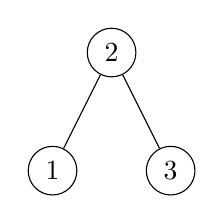
\begin{tikzpicture}[nodes={draw, circle}, -]
    \node{2}
    child { node {1} }
    child { node {3} };
    \end{tikzpicture}
    \caption{An undirected labelled graph with 3 nodes, $\mathcal{V}=\left\lbrace1,2,3\right\rbrace$ and $\mathcal{E}=\left\lbrace\left\lbrace1,2\right\rbrace\left\lbrace2,3\right\rbrace\right\rbrace$.}
    \label{fig:und_graph}
\end{figure} $\newline$
The \textit{neighbours} of node $i$ are defined as all nodes in $\mathcal{G}$ with an edge to node $i$,
\begin{equation*}
    \hbox{ne}\left(i\right)=\left\lbrace j\in\mathcal{V}:\left\lbrace i,j\right\rbrace\in\mathcal{E}\right\rbrace.
\end{equation*}
This definition can be extended to a set $A\subset\mathcal{V}$, where the neighbours of $A$ are defined as
\begin{equation*}
    \hbox{ne}\left(A\right)=\bigcup_{i\in A}\hbox{ne}\left(i\right)\setminus A.
\end{equation*}
A \textit{path} from $i_1$ to $i_m$ is defined as a sequence of certain nodes in $\mathcal{V}, i_1,i_2,...,i_m$, for which $\left(i_j,i_{j+1}\right)\in\mathcal{E}$ for $j=1,...,m-1$. Two nodes $i\notin C$ and $j\notin C$ are \textit{separated} by a subset $C\subset\mathcal{V}$, if every path from $i$ to $j$ contains at least one node from $C$. Two disjoint sets $A\subset\mathcal{V}\notin C$ and $B\subset\mathcal{V}\notin C$ are separated by $C$, if all $i\in A$ and $j\in B$ are separated by $C$, that is, it is not possible to "wander" on the graph from somewhere in $A$ and end somewhere in $B$ without crossing $C$.\\
If $i$ and $j$ are neighbours in $\mathcal{G}$, this can be expressed by $i\overset{\mathcal{G}}{\sim}j$ or $i\sim j$ for the case where the graph is implicit. It follows that $i\sim j\Longleftrightarrow j\sim i$. \\
Let $A$ be a subset of $\mathcal{V}$. A \textit{subgraph} $\mathcal{G}^A$ is a graph restricted to $A$, i.e., the graph obtained after removing all nodes that do not belong to $A$ and all edges where at least one node does not belong to $A$. $\mathcal{G}^A=\left\lbrace\mathcal{V}^A,\mathcal{E}^A\right\rbrace$, where $\mathcal{V}^A=A$ and 
\begin{equation*}
    \mathcal{E}^A = \left\lbrace\left\lbrace i,j\right\rbrace\in\mathcal{A} \hbox{ and } \left\lbrace i,j\right\rbrace\in A\times A\right\rbrace.
\end{equation*}
Let $\mathcal{G}$ be the graph in \autoref{fig:und_graph} and $\mathcal{A}=\left\lbrace2,3\right\rbrace$, then $\mathcal{V}^A=\left\lbrace2,3\right\rbrace$ and $\mathcal{E}^A=\left\lbrace\left\lbrace 2,3\right\rbrace\right\rbrace$ \autocite[][17--18]{rue2005gaussian}.
\subsection{Notation and Basic Properties}
\label{sec:notation}
For structured additive regression models, the distribution of the response variable $y_i$ is assumed to be a member of the exponential family, with the mean $\mu_i$ linked to a structured additive predictor $\eta_i$ by a link function $g\left(\cdot\right)$ such that $g\left(\mu_i\right)=\eta_i$. Following \cite{stone1985additive}, the predictor $\eta_i$  takes into account the effect of multiple covariates in an additive way,
\begin{equation}\label{eq:predictor}
    \eta_i=\alpha+\sum_{j=1}^{n_f}f^{(j)}\left(u_{ji}\right)+\sum_{k=1}^{n_{\beta}}\beta_kz_{ki}+\epsilon_i, \hspace{20pt}i=1,...,n.
\end{equation}
The $\left\lbrace f^{(j)}\left(\cdot\right)\right\rbrace$s are unknown functions of the covariates $u$, while the $\left\lbrace\beta_k\right\rbrace$s represent the linear effect of the covariates $z$ and the $\epsilon_i$s are unstructured terms. Latent Gaussian models assign a Gaussian prior to $\alpha$, $\left\lbrace f^{(j)}\left(\cdot\right)\right\rbrace$ and $\left\lbrace\epsilon_i\right\rbrace$. In the following $\pmb{x}$ shall denote the vector of all latent Gaussian variables ($\left\lbrace\eta_i\right\rbrace$, $\alpha$, $\left\lbrace f^{(j)}\right\rbrace$ and $\left\lbrace\beta_k\right\rbrace$) and $\pmb{\theta}$ the vector of hyperparameters.\\
The conditional density $\pi\left(\pmb{x}|\theta_1\right)$ is Gaussian with an assumed zero mean and precision matrix $\pmb{Q}\left(\theta_1\right)$. The Gaussian density $\mathcal{N}\left(\mu,\pmb{\Sigma}\right)$ with mean $\mu$ and covariance $\pmb{\Sigma}$ at configuration $\pmb{x}$ is denoted by $\mathcal{N}\left(\pmb{x};\mu,\pmb{\Sigma}\right)$. For simplicity, $\left\lbrace\eta_i\right\rbrace$ is included instead of $\left\lbrace\epsilon_i\right\rbrace$. \\
The distribution for the $n_d$ observational variables $y=\left\lbrace y_i:i\in\mathcal{I}\right\rbrace$ is denoted by $\pi\left(\pmb{y}|\pmb{x}, \theta_2\right)$ and is assumed conditionally independent given $\pmb{x}$ and $\theta_2$. Let $\pmb{\theta}=\left(\theta_1^T,\theta_2^T\right)^T$ with $\dim\left(\pmb{\theta}\right)=m$. Following \cite{rue2009approximate}, for non-singular $\pmb{Q}\left(\pmb{\theta}\right)$ the posterior is given by
\begin{align}
    \pi\left(\pmb{x},\pmb{\theta}|\pmb{y}\right)&\propto\pi\left(\pmb{\theta}\right)\pi\left(\pmb{x}|\pmb{\theta}\right)\prod_{i\in I}\pi\left(y_i|x_i,\pmb{\theta}\right) \nonumber\\
    &\propto \pi\left(\pmb{\theta}\right)\left|\pmb{Q}\left(\pmb{\theta}\right)\right|^{1/2}\exp\left[-\frac{1}{2}\pmb{x}^T\pmb{Q}\left(\pmb{\theta}\right)\pmb{x}+\sum_{i\in I}\log\left\lbrace\pi\left(y_i|x_i,\pmb{\theta}\right)\right\rbrace\right].
\end{align}
\subsection{Definition of GMRFs}
Let $\pmb{x}=\left(x_1,...,x_n\right)^T$ be normally distributed with mean $\pmb{\mu}$ and covariance matrix $\pmb{\Sigma}$. Let $\mathcal{G}=\left(\mathcal{V}, \mathcal{E}\right)$, where $\mathcal{V}=\left\lbrace 1,...,\right\rbrace$ and $\mathcal{E}$ be such that there is no edge between nodes $i$ and $j$ exactly when $x_i\perp x_j|\pmb{x}_{ij}$. Then $\pmb{x}$ is a \textit{Gaussian Markov random field} (GMRF) with respect to $\mathcal{G}$. \\
Since $\pmb{\mu}$ does not affect the pairwise conditional independence properties of $\pmb{x}$, this information is 'hidden' in $\pmb{\Sigma}$. Hence,
\begin{equation*}
    x_i\perp x_j|x_{ij}\Longleftrightarrow Q_{ij}=0.
\end{equation*}
Therefore, the non-zero pattern of $\pmb{Q}$ determines $\mathcal{G}$, i.e. whether $x_i$ and $x_j$ are conditionally independent, and can be derived from $\pmb{Q}$. If $\pmb{Q}$ is a fully dense matrix, $\mathcal{G}$ is fully connected, implying that any normal distribution with SPD covariance matrix is a GMRF and vice versa. \\
The elements of $\pmb{Q}$ are used for conditional interpretations. For any GMRF with respect to $\mathcal{G}=\left(\mathcal{V}, \mathcal{E}\right)$ with mean $\pmb{\mu}$ and precision matrix $\pmb{Q} > 0$,
\begin{align}
    \mathbb{E}\left[x_i|\pmb{x}_{-i}\right] &= \mu_i-\frac{1}{Q_{ii}}\sum_{j:j\sim i}Q_{ij}\left(x_j-\mu_j\right), \label{eq:mean_gmrf}\\
    \hbox{Prec}\left(x_i|\pmb{x}_{-i}\right) &= Q_{ii} \hspace{20pt}\hbox{ and }\label{eq:prec_gmrf}\\
    \hbox{Corr}\left(x_i,x_j|\pmb{x}_{ij}\right) &= -\frac{Q_{ij}}{\sqrt{Q_{ii}Q_{jj}}},\hspace{20pt} i\neq j
\end{align}
\autocite[][21]{rue2005gaussian}. \\
On the main diagonal of $\pmb{Q}$ are the conditional precisions of $x_i$ given $\pmb{x}_{-i}$ are placed, while the other elements, when scaled appropriately, provide information about the conditional correlation between $x_i$ and $x_j$ given $\pmb{x}_{ij}$. Since $\hbox{Var}\left(x_i\right)=\Sigma_{ii}$ and $\hbox{Corr}\left(x_i,x_j\right)=\Sigma_{ij}/\sqrt{\Sigma_{ii}\Sigma_{jj}}$, the information about the marginal variance of $x_i$ and the marginal correlation between $x_i$ and $x_j$ is given by $\pmb{\Sigma}$. The marginal interpretation provided by the correlation matrix is intuitive and informative, as the scope of the interpretation is reduced from a $n$-dimensional distribution to a one- or two-dimensional distribution. $\pmb{Q}$ is difficult to interpret marginally because either $\pmb{x}_{-i}$ or $\pmb{x}_{ij}$ would have to be integrated out of the joint distribution parameterized with respect to $\pmb{Q}$. $\pmb{Q}^{-1}=\pmb{\Sigma}$ by definition, and in general $\Sigma_{ii}$ depends on each element in $\pmb{Q}$ and vice versa \autocite[][20--23]{rue2005gaussian}.
\subsection{Markov Properties of GMRFs}
One property of GMRFs is that more information regarding conditional independence can be extracted from $\mathcal{G}$. The following three properties are equivalent. \\
The \textit{pairwise Markov property}:
\begin{equation*}
    x_i\perp x_j|\pmb{x}_{ij}\hspace{20pt}\hbox{ if }\left\lbrace i,j\right\rbrace\notin\mathcal{E}\hbox{ and }i\neq j.
\end{equation*}
The \textit{local Markov property}:
\begin{equation*}
    x_i\perp \pmb{x}_{-\left\lbrace i, \hbox{ne}\left(i\right)\right\rbrace}|\pmb{x}_{\hbox{ne}\left(i\right)}\hspace{20pt}\forall i\in\mathcal{V}.
\end{equation*}
The \textit{global Markov property}:
\begin{equation*}
    \pmb{x}_{A}\perp \pmb{x}_{B}|\pmb{x}_{C}
\end{equation*}
for all disjoint sets $A$, $B$ and $C$ where $A$ and $B$ are non-empty and separated by $C$. \\ \clearpage Illustrations for these properties are shown in Figure~\ref{fig:pairwise}, Figure~\ref{fig:local} and Figure~\ref{fig:global}. These illustrations are taken from Rue and Held \autocite[][23--24]{rue2005gaussian}.
\begin{figure}[H]
    \centering
    \ctikzfig{ind_fig1}
    \caption{The pairwise Markov property; the black nodes are conditionally independent given the light grey nodes.}
    \label{fig:pairwise}
\end{figure}
\begin{figure}[H]
    \centering
    \ctikzfig{ind_fig2}
    \caption{The local Markov property; the black nodes and white nodes are conditionally independent given the dark grey nodes.}
    \label{fig:local}
\end{figure}
\begin{figure}[H]
    \centering
    \ctikzfig{ind_fig3}
    \caption{The global Markov property; the dark grey and light grey nodes are globally independent given the black nodes.}
    \label{fig:global}
\end{figure}
\subsection{Conditional Properties of GMRFs}
An essential result of GMRFs is the conditional distribution for a subset $\pmb{x}_a$ given $\pmb{x}_{-A}$. Here the canonical parameterization proves useful, since by definition it can be easily updated by successive conditioning. \clearpage
By splitting the indices into the non-empty sets A and B, of which the latter is equal to -A,
\begin{equation}\label{eq:partition_1}
    \pmb{x}=\begin{pmatrix}\pmb{x}_A\\\pmb{x}_B\end{pmatrix}.
\end{equation}
The mean and the precision are divided accordingly,
\begin{equation}\label{eq:partition_2}
    \pmb{\mu}=\begin{pmatrix}\pmb{\mu}_A\\\pmb{\mu}_B\end{pmatrix},\hspace{20pt}\hbox{ and }\hspace{20pt}\pmb{Q}=\begin{pmatrix}\pmb{Q}_{AA} & \pmb{Q}_{AB} \\ \pmb{Q}_{BA} & \pmb{Q}_{BB}\end{pmatrix}.
\end{equation}
The conditional distribution of $\pmb{x}_A|\pmb{x}_B$ is a GMRF with respect to the subgraph $\mathcal{G}^A$ with mean $\pmb{\mu}_{A|B}$ and precision matrix $\pmb{Q}_{A|B}>0$, where
\begin{equation}
    \pmb{\mu}_{A|B}=\pmb{\mu}_A-\pmb{Q}_{AA}^{-1}\pmb{Q}_{AB}\left(\pmb{x}_B-\pmb{\mu}_B\right)
\end{equation}
and
\begin{equation*}
    \pmb{Q}_{A|B}=\pmb{Q}_{AA}.
\end{equation*}
Thus, the explicit knowledge of $\pmb{Q}_{A|B}$ is available through $\pmb{Q}_{AA}$, i.e. no calculation is required to obtain the conditional precision matrix. Moreover, the conditional mean depends only on the values of $\pmb{\mu}$ and $\pmb{Q}$ in $A\cup\,\hbox{ne}\left(A\right)$, since $Q_{ij} = 0\,\forall j\not in\hbox{ne}\left(i\right)$. \\
For successive conditioning, the canonical parameterization for GMRF is useful. \\
A GMRF $\pmb{x}$ with respect to $\mathcal{G}$ and canonical parameters $\pmb{b}$ and $\pmb{Q}>0$ has the density
\begin{equation*}
    \pi\left(\pmb{x}\right)\propto\exp\left(-1\frac{1}{2}\pmb{x}^T\pmb{Q}\pmb{x}+\pmb{b}^T\pmb{x}\right).
\end{equation*}
The precision matrix is $\pmb{Q}$ and the mean is $\pmb{\mu}=\pmb{Q}^{-1}\pmb{b}$. The canonical parameterization is written as 
\begin{equation*}
    \pmb{x}\sim \mathcal{N}_C\left(\pmb{b},\pmb{Q}\right).
\end{equation*}
Furthermore,
\begin{equation*}
    \mathcal{N}\left(\pmb{\mu},\pmb{Q}^{-1}\right) \Longleftrightarrow \mathcal{N}_C\left(\pmb{Q\mu}, \pmb{Q}\right).
\end{equation*}
If the indices are partitioned into two non-empty sets A and B and $\pmb{x}$, $\pmb{b}$ and $\pmb{Q}$ are partitioned as in \eqref{eq:partition_1} and \eqref{eq:partition_2}, then
\begin{equation}
    \pmb{x}_A|\pmb{x}_B\sim\mathcal{N}_C\left(\pmb{b}_A-\pmb{Q}_{AB}\pmb{x}_B,\pmb{Q}_{AA}\right).
\end{equation}
Let $\pmb{y}|\pmb{x}\sim\mathcal{N}\left(\pmb{x},\pmb{P}^{-1}\right)$ and $\pmb{x}\sim\mathcal{N}_C\left(\pmb{b},\pmb{Q}\right)$, then
\begin{equation}
    \pmb{x}|\pmb{y}\sim\mathcal{N}_C\left(\pmb{b}+\pmb{Py}, \pmb{Q}+\pmb{P}\right).
\end{equation}
This allows the calculation of conditional densities with multiple sources of conditioning, e.g. conditioning on observed data and a subset of variables. Therefore, the canonical parameterization can be repeatedly updated without explicitly calculating the mean until it is needed. The computation of the mean requires the solution of $\pmb{Q\mu}=\pmb{b}$, but only matrix-vector products are needed for updating the canonical parameterization \autocite[][25--27]{rue2005gaussian}.
\subsection{Specification Through Full Conditionals}
Alternatively, a GMRF can be specified by the full conditionals $\left\lbrace\pi\left(x_i|\pmb{x}_{-i}\right)\right\rbrace$ in place of $\pmb{\mu}$ and $\pmb{Q}$. Suppose the full conditionals are given as normals with
\begin{align}
    \mathbb{E}\left[x_i|\pmb{x}_{-i}\right] &= \mu_i-\sum_{j:j\sim i}\beta_{ij}\left(x_j-\mu_j\right)\hspace{20pt}\hbox{ and}\\
    \hbox{Prec}\left(x_i|\pmb{x}_{-i}\right) &= \kappa_i>0
\end{align}
for $i=1,...,n$, for $\pmb{\mu}$, $\pmb{\kappa}$ and some $\left\lbrace\eta_{ij},i\neq j\right\rbrace$. Evidently, $\sim$ is implicitly defined by the non-zero terms of $\left\lbrace\beta_{ij}\right\rbrace$. For there to exist a joint density $\pi\left(\pmb{x}\right)$ leading to these full conditional distributions, these full conditionals must be consistent. Since $\sim$ is symmetric, it follows that if $\beta_{ij}\neq 0$, then $\beta_{ji}\neq0$. If the entries of the precision matrix are chosen such that
\begin{equation*}
    Q_{ii}=\kappa_i, \hspace{20pt}\hbox{ and }\hspace{20pt} Q_{ij}=\kappa_i\beta_{ij}
\end{equation*}
and $\pmb{Q}$ must be symmetrical, i.e.,
\begin{equation*}
    \kappa_i\beta_{ij}=\kappa_j\beta_{ji},
\end{equation*}
then $\pmb{x}$ is a GMRF with respect to a labelled graph $\mathcal{G}=\left(\mathcal{V}, \mathcal{E}\right)$ with mean $\pmb{\mu}$ and precision matrix $\pmb{Q}=\left(Q_{ij}\right)$ \autocite[][27]{rue2005gaussian}.
\subsection{Lattices and Tori}
$\mathcal{I}_{\pmb{n}}$ denotes a (regular) \textbf{lattice} (or grid) of size $\pmb{n}=\left(n_1, n_2\right)$ (in the two-dimensional case). $\pmb{y}$ can take values on $\mathcal{I}_{\pmb{n}}$ and $y_{i,j}$ denotes the value of $\pmb{y}$ at location $ij$, for $i=1,...,n_1$ and $j=1,...,n_2$. For easier reading this is shortened to $y_{ij}$. On an \textit{infinite lattice} $\mathcal{I}_{\pmb{\infty}}$, $ij$ are numbered as $i=0,\pm1,\pm2,...,$ and $j=0,\pm1,\pm2,...$. \\
A lattice with cyclic or toroidal boundary conditions is referred to as \textit{torus} and is denoted by $\mathcal{I}_{\pmb{\infty}}$. The dimension is $\pmb{n}=\left(n_1,n_2\right)$ (in the two-dimensional case) and all indices are modulus $\pmb{n}$ and run from 0 to $n_1-1$ or $n_2-1$. If a GMRF $\pmb{y}$ is defined on $\mathcal{I}_{\pmb{n}}$, the toroidal boundary conditions imply that $y_{-2,n_2}$ is equal to $y_{n_1-2,0}$ since $-2\mod n_1$ is equal to $n_1-2$ and $n_2\mod n_2$ is equal to 0.\\
An \textit{irregular lattice} refers to a spatial configuration of regions $i=1,...,n$ where the regions (mostly) have common boundaries, for instance the states of a nation \autocite[][15--16]{rue2005gaussian}. An example of an irregular lattice is shown in Figure~\ref{fig:lattice}.
\begin{figure}[H]
   \centering
       \includegraphics[page=1,width=\textwidth]{switzerland.pdf}
 \caption{The cantons of Switzerland, an example of an irregular lattice.}
 \label{fig:lattice}
\end{figure}
\clearpage
\section{Latent Gaussian Models and INLA}
In recent years, a growing amount of georeferenced data has become available, leading to an increased need for appropriate statistical modelling to handle large and complex datasets. The usual approach to inference in this field involves the previously introduced Markov chain Monte Carlo methods. Due to several factors, these methods may perform poorly when applied to such models. One issue is the high dependence from $\pmb{\theta}$ and $\pmb{x}$ on each other, especially for large $n$. This problem requires, at least in part, a joint update of $\pmb{\theta}$ and $\pmb{x}$. There are several proposals to solve these shortcomings, but MCMC sampling continues to show poor computational speed \autocite[][322]{rue2009approximate}.\\
Bayesian hierarchical models have proven to be effective in capturing complex stochastic structures in spatial processes. A large proportion of these models are based on latent Gaussian models, a subclass of structured additive regression models. The methodology used for these models includes Integrated Nested Laplace Approximations (INLA), which is a method used to approximate the posterior marginals of a latent Gaussian field and hyperparameters $\pmb{\theta}$. The hyperparameters $\pmb{\theta}$ can be, for example, the variance in the Gaussian likelihood or the shape parameter in the likelihood of the gamma distribution. In the case of latent fields, they can be, for instance, dispersion parameters or spatial correlation parameters. 
Most latent Gaussian models satisfy two basic properties:
\begin{itemize}
    \item[1.] The latent field $\pmb{x}$ is of large dimension, $n\approx10^2-10^5$. Therefore, the latent field is a Gaussian Markov random field with sparse precision matrix $\pmb{Q}\left(\pmb{\theta}\right)$.
    \item[2.] The number of hyperparameters, $m$, is small, $m\leq6$.
\end{itemize}
In most cases, both properties are required to produce fast inference, and thus these are assumed to be true for the remainder of this work \autocite[][]{rue2009approximate}.
\subsection{Applications for Latent Gaussian Models}
Latent Gaussian models can be employed in a vast range of different domains, in fact most structured Bayesian models are of this particular form. Some of these domains are presented next. \clearpage
\subsubsection{Regression Models}
Bayesian generalized linear models correspond to the linear relationship $\eta_i=\alpha+\sum_{k=1}^{n_\beta}\beta_k z_{ki}$ \autocite[][]{dey2000generalized}. Either the linear relationship of the covariates can be relaxed through the $f\left(\cdot\right)$ terms \autocite[][]{fahrmeir2013multivariate}, random effects can be introduced through them or both. Smooth covariate effects are frequently modelled using penalized spline models \autocite[][]{lang2004bayesian} or random walk models \autocite[][]{fahrmeir2013multivariate}, continuous indexed spline models \autocite[][]{rue2005gaussian} or Gaussian processes \autocite[][]{chu2005gaussian}. The incorporation of random effects allows for the consideration of overdispersion caused by unobserved heterogeneity or correlation in longitudinal data and can be introduced by defining $f\left(u_i\right)=f_i$ and $\left\lbrace f_1\right\rbrace$ to be independent, zero mean and Gaussian \autocite[][]{fahrmeir2001bayesian}.
\subsubsection{Dynamic Models}
Temporal dependence can be introduced by using $i$ in \eqref{eq:predictor} as temporal index $t$ and defining $f\left(\cdot\right)$ and $\pmb{u}$ such that $f\left(u_t\right)=f_t$. Both a discrete-time and a continuous-time autoregressive model can be modelled by $\left\lbrace f_t\right\rbrace$. Furthermore, a seasonal effect or the latent process of a structured time series model can be modelled \autocite[][]{kitagawa1996smoothness}. Alternatively, a smooth temporal function in the same sense as for regression models can be represented by $\left\lbrace f_t\right\rbrace$.
\subsubsection{Spatial and Spatio-Temporal Models}
Similar to the previous type of model, spatial dependence can be modelled by a spatial covariate $\pmb{u}$ such that $f\left(u_s\right)=f_s$, where $s$ denotes the spatial location or region $s$. The stochastic model for $f_s$ is constructed to promote spatial smooth realizations of some sort. Popular models of this type include the Besag-York-Mollié \autocite[][]{besag1991bayesian} model with extensions for regional data, continuous indexed Gaussian models \autocite[][]{banerjee2014hierarchical} and texture models \autocite[][]{marroquin2001gauss}. The dependence between spatial and temporal covariates can be achieved either by using a spatio-temporal covariate $(s,t)$ or a corresponding spatio-temporal Gaussian field \autocite[][]{kammann2003geoadditive}.\\
Often the final model consists of a sum of several components, e.g. a spatial component, random effects and both linear and smooth effects of some covariates. In order to separate the effects of the different components in \eqref{eq:predictor}, sometimes linear or sum-to-zero constraints can be imposed \autocite[][319--321]{rue2009approximate}.
\subsection{Integrated Nested Laplace Approximation}
An alternative to MCMC methods that is both less computationally intensive and suitable for performing approximate Bayesian inference in latent Gaussian models is \textit{Integrated Nested Laplace Approximation} (INLA). The basis of INLA is the use of a combination of analytical approximations and numerical algorithms for sparse matrices to approximate the posterior distribution using closed-form expressions. This speeds up inference and circumvents problems of sample convergence and mixing, making it suitable for fitting large data sets or exploring other models \autocite[][]{rue2009approximate}.  \\
INLA can be used for all models of the following form,
\begin{align*}
    y_i|\pmb{x},\pmb{\theta} &\sim \pi\left(y_i|x_i,\pmb{\theta}\right), \hspace{20pt} i=1,...,n,\\
    \pmb{x}|\pmb{\theta} &\sim \mathcal{N}\left(\mu\left(\pmb{\theta}\right), \pmb{Q}\left(\pmb{\theta}\right)^{-1}\right), \\
    \pmb{\theta} &\sim \pi\left(\pmb{\theta}\right).
\end{align*}
As introduced in \autoref{sec:notation}, $\pmb{y}$ are the observed data, $\pmb{x}$ is a Gaussian field, $\pmb{\theta}$ represents the hyperparameters, while $\mu\left(\pmb{\theta}\right)$ and $\pmb{Q}\left(\pmb{\theta}\right)$ denote the mean and precision matrix respectively. To ensure fast inference, the dimension of the hyperparameter vector $\pmb{\theta}$ should be small, since the approximations are computed by numerical integration over the hyperparameter space. \\
In most cases, the observations $y_i$ are assumed to belong to the exponential family with mean $\mu_i=g^{-1}\left(\eta_i\right)$. As shown in equation \eqref{eq:predictor}, $\eta_i$ accounts for the effects of several covariates in an additive way, which makes it suitable for a wide range of models, including spatial and spatio-temporal models, since $\left\lbrace f^{(j)}\right\rbrace$ can take different forms. \\
Let $\pmb{x}$ be a GMRF, and let $\pmb{\theta}$ be the vector of hyperparameters, which are not required to be Gaussian. INLA calculates accurate and fast approximations for the posterior marginals of the components of the latent Gaussian variables
\begin{equation*}
    \pi\left(x_i|\pmb{y}\right),\hspace{20pt}i=1,...,n,
\end{equation*}
as well as the posterior marginals for the hyperparameters of the latent Gaussian model
\begin{equation*}
    \pi\left(\theta_j|\pmb{y}\right),\hspace{20pt}j=1,...,\dim\left(\pmb{\theta}\right).
\end{equation*}
For each element $x_i$ of $\pmb{x}$ the posterior marginals are given by
\begin{equation}
    \pi\left(x_i|\pmb{y}\right)=\int\pi\left(x_i|\pmb{\theta},\pmb{y}\right)\pi\left(\pmb{\theta}|\pmb{y}\right)d\pmb{\theta},
\end{equation}
and the posterior marginal for the hyperparameters can be expressed by
\begin{equation}
    \pi\left(\theta_j|\pmb{y}\right)=\int\pi\left(\pmb{\theta}|\pmb{y}\right)d\pmb{\theta}_{-j}.
\end{equation}
$\pi\left(x_i|\pmb{y}\right)$ is approximated by combining analytical approximations to the full conditionals $\pi\left(x_i|\pmb{\theta},\pmb{y}\right)$ and $\pi\left(\pmb{\theta}|\pmb{y}\right)$ and numerical integration routines to integrate out $\pmb{\theta}$. Similarly, $\pi\left(\theta_j|\pmb{y}\right)$ is approximated by approximating $\pi\left(\pmb{\theta}|\pmb{y}\right)$ and integrating out $\pmb{\theta}_{-j}$. In particular, the posterior density of $\pmb{\theta}$ is obtained through Gaussian approximation for the posterior of the latent field, $\widetilde{\pi}_G\left(\pmb{x}|\pmb{\theta},\pmb{y}\right)$, evaluated at the posterior mode, $x^*\left(\pmb{\theta}\right)=\arg\max_{\pmb{x}}\pi_G\left(\pmb{x}|\pmb{\theta},\pmb{y}\right)$,
\begin{equation}
    \widetilde{\pi}\left(\pmb{\theta}|\pmb{y}\right)\propto\frac{\pi\left(\pmb{x},\pmb{\theta},\pmb{y}\right)}{\widetilde{\pi}_G\left(\pmb{x}|\pmb{\theta},\pmb{y}\right)}\bigg|_{\pmb{x}=x^*\left(\pmb{\theta}\right)}.
\end{equation}
Next, the following nested approximations are constructed,
\begin{equation}
    \widetilde{\pi}\left(x_i|\pmb{y}\right)=\int\widetilde{\pi}\left(x_i|\pmb{\theta},\pmb{y}\right)\widetilde{\pi}\left(\pmb{\theta}|\pmb{y}\right)d\pmb{\theta},\hspace{20pt}\widetilde{\pi}\left(\theta_j|\pmb{y}\right)=\int\widetilde{\pi}\left(\pmb{\theta}|\pmb{y}\right)d\pmb{\theta}_{-j}.
\end{equation}
Finally, these approximations are numerically integrated with respect to $\pmb{\theta}$
\begin{align}
    \widetilde{\pi}\left(x_i|\pmb{y}\right)&=\sum_k\widetilde{\pi}\left(x_i|\theta_k,\pmb{y}\right)\widetilde{\pi}\left(\theta_k|\pmb{y}\right)\times\Delta_k,\\
    \widetilde{\pi}\left(\theta_j|\pmb{y}\right)&=\sum_l\widetilde{\pi}\left(\theta_l^*|\pmb{y}\right)\times\Delta_l^*,
\end{align}
with $\Delta_k$ and $\Delta_l^*$ representing the area weights corresponding to $\theta_k$ and $\theta_l^*$. \\
To obtain the approximations for the posterior marginals for the $x_i$'s conditioned on selected values of $\theta_k$ and $\widetilde{\pi}\left(x_i|\theta_k,\pmb{y}\right)$, a Gaussian, Laplace or simplified Laplace approximation can be used. Using a Gaussian approximation derived from $\widetilde{\pi}_G\left(\pmb{x}|\pmb{\theta},\pmb{y}\right)$ is the simplest and fastest solution, but in some situations it produces errors in the location and is unable to capture skewness behaviour. Therefore, the Laplace approximation is favoured over the Gaussian approximation, although it is relatively expensive. The simplified Laplace approximation is associated with lower costs and addresses inaccuracies of the Gaussian approximation in terms of location and skewness in a satisfactory manner \autocite[][]{rue2009approximate, rue2017bayesian}.
\clearpage
\section{Bayesian Spatial Models}
Bayesian spatial models are often used in the field of disease mapping. Bayesian hierarchical
models improve estimates of log risk by providing information about neighbouring regions in the spatially structured component as well as regional variation in the unstructured component \autocite[][]{blangiardo2015spatial}. One of the most well-known spatial models is Besags' spatial model, which is presented in Section~\ref{sec:besag}. Several models have been developed based on the Besag model, including the Besag-York-Mollié (BYM) model, introduced in Section~\ref{sec:bym}, the Leroux model, introduced in Section~\ref{sec:leroux}, and more recently the BYM2 model, introduced in Section~\ref{sec:bym2}. \\
In general, it can be assumed that areas in proximity to each other have a more frequent burden of disease than areas that are further away from each other. By setting up a neighbourhood structure, this "proximity" can be defined. It is assumed that $i$ and $j$ are neighbours if they share a common boundary, denoted $i\sim j$. The set of neighbours of the region $i$ is denoted by $\delta_i$ and its size is given by $n_{\delta_i}$.
\subsection{Besag Spatial Models}\label{sec:besag}
\subsubsection{Besags' Improper Spatial Model}
A commonly used approach to modelling spatial correlation is the Besag model, also known as an intrinsic or improper GMRF model. The conditional distribution for a random vector $\pmb{x}=\left(x_1,...,x_n\right)^T$ is given by
\begin{equation}
    x_i|\pmb{x}_{-i},\tau_x\sim\mathcal{N}\left(\frac{1}{n_{\delta_i}}\sum_{j\in\delta_i}x_j,\frac{1}{n_{\delta_i}\tau_x}\right),
\end{equation}
with $\tau_x$ as a precision parameter. The mean of the effects over all neighbours is given by the mean of $x_i$, while the precision is proportional to the number of neighbours. The joint distribution for $\pmb{x}$ is given by
\begin{equation}
    \pi\left(\pmb{x}|\tau_x\right)\propto\exp\left(-\frac{\tau_x}{2}\sum_{i\sim j}\left(x_i-x_j\right)^2\right)\propto\exp\left(-\frac{\tau_x}{2}\pmb{x}^T\pmb{Q}\pmb{x}\right).
\end{equation} \clearpage
The precision matrix $\pmb{Q}$ is given by
\begin{equation}
    Q_{ij}=\begin{cases}
    n_{\delta_i}&i=j,\\
    -1&i\sim j,\\
    0&\hbox{else.}
    \end{cases}
\end{equation}
\pmb{Q} is a singular matrix, i.e. it has a non-empty null space $\pmb{V}$, hence the model is called intrinsic or Besags' improper spatial model. \\
The Besag model for spatial effects has one hyperparameter, the precision $\tau_x$, which is represented as
\begin{equation}
    \theta_1 = \log\tau_x.
\end{equation}
The prior is defined on $\theta_1$. This model implies that the conditional expected value of $x_i$ is equivalent to the mean of the random effects at the neighbouring locations \autocite[][]{besag1974spatial, riebler2016intuitive}.
\subsubsection{Besags' Proper Spatial Model}
Since the joint distribution of the intrinsic Besag model is improper due to the singular precision matrix, this impropriety can be overcome by redefining the precision matrix as follows,
\begin{equation}
    Q_{ij} = \begin{cases}
    \tau_x\left(n_{\delta_i}+d\right) & i=j,\\
    -\tau &\hbox{else.}
    \end{cases}
\end{equation}
$d > 0$  is an additional term added to the diagonal to control the "properness". The conditional distribution for the proper version of the Besag model is given by
\begin{equation}
    x_i|\pmb{x}_{-i},\tau_x,d\sim\mathcal{N}\left(\frac{1}{d+n_{\delta_i}}\sum_{i\sim j}x_j\frac{1}{\tau_x\left(d+n_{\delta_i}\right)}\right).
\end{equation}
The proper version of the Besag model for spatial effects has two hyperparameters, the precision $\tau_x$, which is represented as
\begin{equation}
    \theta_1 = \log\tau_x
\end{equation}
and the diagonal parameter $d$, which is represented as
\begin{equation}
    \theta_2 = \log d.
\end{equation}
The priors are defined on $\theta_1$ and $\theta_2$, respectively \autocite[][]{besag1974spatial, riebler2016intuitive}.
\subsection{The Besag-York-Mollié Model}\label{sec:bym}
The Besag-York-Mollié (BYM) model is a lognormal Poisson model that is a combination of an improper Besag model $u$ and an ordinary random effect component $v$ for non-spatial heterogeneity. It combines the regional spatial effect $\pmb{x}$ into the sum of an unstructured and a structured spatial component, so that $\pmb{x}=\pmb{v}+\pmb{u}$.\\
$\pmb{v}\sim\mathcal{N}\left(0,\tau_v^{-1}\pmb{I}\right)$ accounts for pure overdispersion, while $\pmb{u}\sim\mathcal{N}\left(\pmb{0}, \tau_u^{-1}\pmb{Q}^{-}\right)$ is the Besag model. \\
By using a spatial and a non-spatial error term, the overdispersion that is not modelled by the Poisson variables is taken into account. Thus, if the observed variance is not fully explained by the spatial structure of the data, the error terms explain the rest of the variance. \\
The resulting covariance matrix of $\pmb{x}$ is given by
\begin{equation}
    \hbox{Var}\left(\pmb{x}|\tau_u,\tau_v\right)=\tau_v^{-1}\pmb{I}+\tau_u^{-1}\pmb{Q}^{-},
\end{equation}
where $\pmb{Q}^{-}$ denotes the generalized inverse of \pmb{Q}. \\
The hyperparameters of the model are the precision $\tau_u$ of the Besag model $u$ and the precision $\tau_v$ of the iid model $v$. They are represented as
\begin{equation}
    \pmb{\theta}=\left(\theta_1, \theta_2\right)=\left(\log\tau_v,\log\tau_u\right)
\end{equation}
and the prior is defined on $\pmb{\theta}$ \autocite[][]{besag1991bayesian, riebler2016intuitive}.
\subsection{The Leroux Model}\label{sec:leroux}
One problem with the BYM model is that the structured and unstructured components are not identifiable because they cannot be considered independently. Moreover, $\tau_v$ and $\tau_u$ do not represent variability at the same level, which makes the choice of hyperpriors difficult. The Leroux model is formulated in such a way that the compromise between the two variations is made more explicit. It is assumed that $\pmb{x}$ follows a normal distribution with zero mean and covariance matrix
\begin{equation}
    \hbox{Var}\left(\pmb{x}|\tau_x,\phi\right)=\tau_x^{-1}\left(\left(1-\phi\right)\pmb{I}+\phi\pmb{Q}\right)^{-1},
\end{equation}
with $\phi\in\left[0,1\right]$ as mixing parameter. For $\phi=0$ the model reduces to pure overdispersion and for $\phi=1$ to the Besag model. The conditional expected value of $x_i$ for all other random effects is the weighted mean of the unstructured model with zero mean and the mean of the Besag model, while the conditional variance is the weighted mean of $\tau_x^{-1}$ and $\left(\tau_x\cdot\ n_{\delta_i}\right)^{-1}$ \autocite[][]{leroux2000estimation, riebler2016intuitive}.
\subsection{The BYM2 Model}\label{sec:bym2}
One problem that all the aforementioned models have is the lack of scaling of the spatially structured component. Scaling facilitates the assignment of hyperpriors and ensures that the interpretation of hyperpriors remains the same across different areas. \\
Another problem is that the marginal standard deviations of the commonly used IGMRF priors can vary greatly, a fact that should be taken into account by assigning hyperpriors to the precision parameters of these models. \\
Since the Besag model penalizes a local deviation from its null space, the hyperprior controls this local deviation and thus affects the smoothness of the estimated spatial effects. If the estimate of the field is too smooth, the precision is large and the spatial variation may be blurred. On the other hand, if the precision is too small, the model could overfit due to the large local variability. \\
The marginal variances $\tau_x^{-1}\left[\pmb{Q}^{-}\right]_{ii}$ depend on the structure of the graph, which is reflected in the structure matrix $\pmb{Q}$. A generalized variance can be calculated as the geometric mean of the marginal variance as follows
\begin{equation}\label{eq:bym_scale}
    \sigma_{\hbox{GV}}^2\left(\pmb{u}\right)=\exp\left(\frac{1}{n}\sum_{i=1}^n\log\left(\frac{1}{\tau_x}\left[\pmb{Q}^{-}\right]_{ii}\right)\right)=\frac{1}{\tau_x}\exp\left(\frac{1}{n}\sum_{i=1}^n\log\left(\left[\pmb{Q}^{-}\right]_{ii}\right)\right).
\end{equation}
In order to unify the interpretation of a chosen prior for $\tau_x$ and make it transferable across domains, the structured effect must be scaled such that $\sigma_{\hbox{GV}}^2\left(\pmb{x}\right)=\tau_x^{-1}$. This implies that $\tau_x$ denotes the accuracy of the (marginal) deviation from a constant level, independent of the underlying graph. \\
A modification of the BYM model that addresses this scaling problem is the BYM2 model. It uses a scaled structured component $\pmb{u}_{*}$, where $\pmb{Q}_{*}$ denotes the precision matrix of the Besag model, scaled with the marginal variance $\sigma_{\hbox{GV}}^2$ as a factor. The random effect is given by
\begin{equation}\label{eq:bym2_1}
    \pmb{x}=\frac{1}{\tau_x}\left(\sqrt{1-\phi}\pmb{v}+\sqrt{\phi}\pmb{u}_{*}\right),
\end{equation}
with covariance matrix
\begin{equation}
    \hbox{Var}\left(\pmb{x}|\tau_x,\phi\right)=\frac{1}{\tau_x}\left(\left(1-\phi\right)\pmb{I}+\phi\pmb{Q}_{*}^{-}\right).
\end{equation} \clearpage
Equation~\ref{eq:bym2_1} emphasizes the trade-off between pure overdispersion and spatially structured correlation, where $0\leq\phi\leq1$ measures the fraction of the marginal variance explained by the structured effect. For $\phi=0$ the model reduces to pure overdispersion, while for $\phi=1$ it becomes a Besag model \autocite[][]{sorbye2017penalised, riebler2016intuitive}.
\clearpage
\section{Prior Sensitivity}\label{sec:issues}
One problem that plagues Bayesian spatial models is that they cannot be directly compared due to their different parameterizations and the fact that the precision in these models is interpreted differently. Since neither a Besag model nor a BYM model nor a Leroux model is scaled, the precision parameter is not representative of the marginal precision but is confounded with the mixing parameter. Therefore, the effect of a prior assigned to the precision parameter is dependent on the graph structure of the application. Thus, a given prior is not transferable between different applications if the underlying graph changes. Furthermore, the goal of the BYM2 model is not to optimize goodness-of-fit indicators, but to provide a meaningful model formulation where all parameters have a clear meaning. By mapping the precision parameter to the marginal standard deviation, the model parameters are flexible and the assignment of meaningful hyperpriors is made easier \autocite[][]{riebler2016intuitive}. \\
Additionally, the goodness-of-fit indicators introduced in Section~\ref{sec:performance} have their own problems. The DIC, for example, produces unreasonable results if the posterior distribution is not well summarized by its mean, while the WAIC is based on a data partition that would create difficulties for structured models, such as for spatial or network data \autocite[][]{gelman2014understanding}. \\
Finally, the choice of the prior affects the value of these criteria and depending on the values chosen for the PC priors used in this work, overfitting of the models may occur, which is reflected in these criteria, but more on this later.